\documentclass[10pt]{article}

\usepackage[letterpaper,margin=0.72in,columnsep=0.26in]{geometry}
\usepackage{amsmath,amssymb,bm,mathtools}
\usepackage{booktabs}
\usepackage{array}
\usepackage{microtype}
\usepackage{setspace}
\usepackage{enumitem}
\usepackage{tikz}
\usepackage[hidelinks]{hyperref}
\usepackage{xcolor}
\usepackage{siunitx}
\usepackage{caption}
\usepackage{balance}

\setstretch{1.08}
\setlength{\parindent}{1.15em}
\setlength{\parskip}{0.18em}
\setlist{nosep,leftmargin=*}
\captionsetup{font=small,labelfont=bf}
\sisetup{detect-all=true}
\raggedbottom
\setlength{\emergencystretch}{2em}

\newcommand{\TEF}{\mathrm{TEF}}
\newcommand{\dd}{\mathrm{d}}
\newcommand{\MSbar}{\overline{\mathrm{MS}}}

\hypersetup{
  pdftitle={From a Gravity-Calibrated Helix to a Strong-Interaction Confinement Correspondence},
  pdfauthor={Xiaodan Wu},
  pdfsubject={The Emergent Frame; closure energetics; strong-interaction confinement correspondence},
  pdfkeywords={The Emergent Frame, confinement, QCD, closure energetics, helical geometry, static potential}
}

\title{\bfseries From a Gravity-Calibrated Helix to a Strong-Interaction Confinement Correspondence}
\author{Xiaodan Wu\textsuperscript{1,*}\\
\small \textsuperscript{1}Independent Researcher\textsuperscript{\(\dagger\)}}
\date{September 6, 2026 --- Version 4.1\\[0.20em]
\small DOI: \href{https://doi.org/10.5281/zenodo.22412464}{10.5281/zenodo.22412464}}

\begin{document}
\twocolumn[
\begin{@twocolumnfalse}
\maketitle
\vspace{-0.7em}
\begin{minipage}{\textwidth}
\small
\begin{center}
\textbf{Abstract}
\end{center}
\noindent
We formulate a conditional closure-energy framework for a restricted connected static-source channel in The Emergent Frame (TEF). The construction joins the inherited open-space helix of Paper I to the matter-closure question of Paper IV without specifying a microscopic quark topology. Closure-compatible states are organized into integer rollout sectors, and a closure-preserving map advances a discrete branch by a fixed separation increment $P$ while increasing the sector count by one. Assuming that this connected branch admits no lower-count shortcut, that the static quadratic form reduces across number sectors, and that the residual energy remains subextensive after optimization over all higher-count sectors, we show that the averaged discrete static-energy slope tends to $\sigma=\Delta E/P$. A separate finite-window bound states the accuracy required before string breaking, while any identification with a continuous-$r$ constrained energy requires additional within-cell control. The TEF specialization sets $P=2\pi n qR_G$; neither $n$ nor the positive increment $\Delta E$ is derived here. A future gauge completion could relate the linear term to rectangular Wilson-loop behavior only under additional spectral and limit assumptions. The result is therefore a conditional statement about connected-channel closure energetics, not a microscopic derivation of QCD confinement. String breaking, flux-tube fluctuations, $SU(3)_c$ dynamics, the numerical origin of $\Delta E$, and ultraviolet running remain unresolved.
\end{minipage}
\vspace{1.25em}
\end{@twocolumnfalse}
]

\begingroup
\renewcommand{\thefootnote}{\fnsymbol{footnote}}
\footnotetext[1]{\href{mailto:xiaodan@theemergentframe.org}{xiaodan@theemergentframe.org}}
\footnotetext[2]{\href{https://theemergentframe.org}{https://theemergentframe.org}; ORCID: 0009-0005-5892-0293.}
\endgroup

\section{Introduction}

Quantum chromodynamics (QCD) describes the strong interaction as an $SU(3)_c$ non-Abelian gauge theory. Its renormalized coupling $\alpha_s(\mu)$ runs with scale according to the QCD beta function, becoming weak at high momentum transfer and nonperturbative at low scales \cite{PDGQCD2025}. In pure gauge theory, and approximately in the connected static-source branch of full QCD before string breaking, the static energy contains a linearly rising contribution,
\begin{equation}
V_{q\bar q}(r)=V_0+\sigma r+\cdots,
\label{eq:qcd_linear}
\end{equation}
where $\sigma$ is the string tension. Lattice calculations have long resolved this behavior in $SU(3)$ gauge theory \cite{BaliSchilling1992}. With dynamical light and strange quarks, modern static-source analyses still extract a lattice-inferred confining reference scale; Bulava \emph{et al.} obtain $\sqrt{\sigma}=445(3)_{\rm stat}(6)_{\rm sys}\,\mathrm{MeV}$ in a model analysis extrapolated to physical light-quark masses \cite{Bulava2024}. Wilson's formulation supplies the standard gauge-theory loop language \cite{Wilson1974}. Effective-string work describes universal corrections, long-range potential structure, and flux-tube spectra beyond the leading tension term \cite{LuscherWeisz2002,Brambilla2014}; recent closed-flux-tube studies in pure-gauge $SU(N_c)$ further resolve nontrivial world-sheet excitations \cite{Athenodorou2025}. In full QCD the connected branch is ultimately limited by string breaking; evidence includes finite-temperature studies \cite{DeTar1999}, zero-temperature $n_f=2$ simulations \cite{BaliStringBreaking2005}, and modern mixed string/two-meson spectra \cite{Bulava2024}.

The present paper asks a narrower structural question than a derivation of QCD: can the existing TEF open-space geometry and matter-closure program be joined by a minimal mathematical interface whose constrained connected-channel energy has a linear static slope under explicit assumptions?

The two antecedents are explicit. Paper I develops the open-space branch through a gravity-calibrated circular-helix ansatz and fixes the dimensionless shape parameter $q$ before later cross-sector tests \cite{WuWeakMixing}. Paper IV develops a complementary matter-topology branch in which quark-like sectors are modeled as locally persistent but globally incomplete sub-sectors of closed matter and identifies the energetics of maintaining closure under separation as a future strong-sector pressure test \cite{WuMatterSpace}. Paper IV does not derive confinement, an energy functional, or a helical matter topology. The present work takes that unresolved pressure test as its starting point.

The strategy is deliberately matter-shape-agnostic. We do \emph{not} specify whether a quark-like sector is a knot, ribbon, tube, network, soliton, or another three-dimensional configuration. Instead we introduce only the abstract ingredients that any future realization would have to implement: a closure condition, a countable open-space rollout operation, and an effective energetic cost for maintaining closure as incomplete sectors separate.

The principal result is a discrete conditional lemma. A closure-preserving raising map carries a connected sector at $(r,N)$ to one at $(r+P,N+1)$, and the branch is assumed to admit no lower-$N$ shortcut. All higher-count sectors are retained in the static energy minimization through an optimized residual envelope. If that full envelope is subextensive relative to the rollout cost, the averaged spectral slope along $r_m=r_0+mP$ tends to $\Delta E/P$. A separate finite-window estimate makes explicit what must already be small in any pre-string-breaking interval. No exact continuous-$r$ conclusion is inferred from smoothness alone: a coarse-grained interpolation is a representation of the discrete result, while the true continuous constrained problem requires an additional within-cell control condition. The TEF helix enters only through $P=P_n=2\pi nqR_G$, and the optional two-turn candidate remains separate from the lemma.

\section{Inherited helix geometry}
\label{sec:inherited}

The present paper inherits the minimal geometric construction of Ref.~\cite{WuWeakMixing}.  A primitive generated spatial line is represented locally by the right-handed circular helix
\begin{equation}
\bm r(\phi)=\bigl(R\cos\phi,\,R\sin\phi,\,a\phi\bigr),
\qquad q\equiv\frac{a}{R}.
\label{eq:helix}
\end{equation}
A complete turn has axial advance
\begin{equation}
P_1=2\pi a=2\pi qR,
\label{eq:p1}
\end{equation}
while the corresponding internal helical arc length is
\begin{equation}
L_1=2\pi R\sqrt{1+q^2}.
\label{eq:l1}
\end{equation}
The earlier construction assigns distinct roles to these lengths: $P_1$ measures net generated axial extension, whereas $L_1$ measures the internal path traversed in one cycle.

The gravity--geometry calibration postulate is
\begin{equation}
G=\frac{8\pi c^3R^2}{h},
\end{equation}
which, when the measured Newton constant is used as input, gives
\begin{equation}
R_G=\sqrt{\frac{hG}{8\pi c^3}}
=\frac{\ell_P}{2}
\simeq 8.0813\times10^{-36}\ \mathrm{m}.
\label{eq:RG}
\end{equation}
A one-cycle phase-closure condition in the earlier model then fixes
\begin{equation}
q\sqrt{1+q^2}=\frac{2}{\pi},
\label{eq:qclosure}
\end{equation}
so that
\begin{equation}
q=0.556324180045\ldots .
\label{eq:qvalue}
\end{equation}
No QCD observable enters Eqs.~\eqref{eq:RG}--\eqref{eq:qvalue}.

The present work uses only $R_G$, $q$, and the distinction between axial rollout and internal helical path.  It does \emph{not} identify the gravitational line-tension scale $c^4/G$ used in the earlier phase construction with the QCD string tension.  The net energy difference between a closed matter configuration and an open spatial configuration is a new dynamical quantity and is left unresolved here. Figure~\ref{fig:two_turn} illustrates only the axial geometry of the optional two-turn specialization; it is not a proposed particle topology.

\begin{figure}[t]
\centering
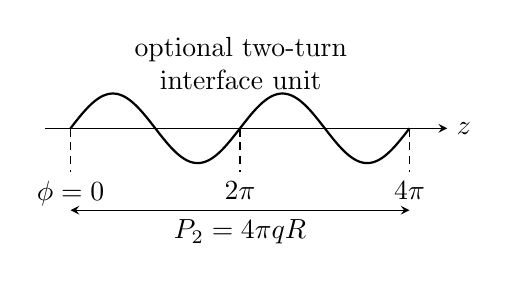
\begin{tikzpicture}[x=0.92cm,y=0.92cm,>=stealth]
  \draw[->] (0.2,0.55) -- (5.75,0.55) node[right] {$z$};
  \draw[thick,domain=0:720,samples=220,smooth,variable=\t]
    plot ({0.55+0.0065*\t},{0.55+0.48*sin(\t)});
  \foreach \x/\lab in {0.55/$\phi=0$,2.89/$2\pi$,5.23/$4\pi$}{
    \draw[densely dashed] (\x,0.55) -- (\x,-0.05);
    \node[below] at (\x,-0.05) {\lab};
  }
  \draw[<->] (0.55,-0.58) -- (5.23,-0.58)
    node[midway,below] {$P_2=4\pi qR$};
  \node[align=center] at (2.9,1.45) {optional two-turn\\interface unit};
\end{tikzpicture}
\caption{Two-dimensional projection of the optional two-turn open-space interface unit. The marked equal-phase points show that $P_2$ is the axial rollout between $\phi=0$ and $4\pi$, not the helical arc length. Handedness is inherited from Eq.~\eqref{eq:helix} and is not encoded by this projection. The figure does not depict a quark or closed-matter topology.}
\label{fig:two_turn}
\end{figure}

\section{Effective closure framework}
\label{sec:opening}

Paper IV introduces a pre-dynamical matter-topology language in which quark-like sectors may be locally persistent yet globally incomplete, while physical composites are associated with a closure condition \cite{WuMatterSpace}. The present paper does not choose a concrete embedding of those sectors. Instead it introduces a minimal effective state-space skeleton that a future microscopic topology may realize.

\subsection{Effective Hilbert space, closure projections, and number sectors}

Let
\begin{equation}
\mathcal H_{\rm eff}=\mathcal H_{\rm M}\otimes\mathcal H_{\rm S}
\label{eq:Heffspace}
\end{equation}
be a formal effective Hilbert space for matter-sector and open-space degrees of freedom. The construction below uses a common dense quadratic-form domain and does not assert that Eq.~\eqref{eq:Heffspace} is fundamental.

For each prescribed separation $r$ in the connected channel, let $\Pi_{\rm cl}(r)$ be a bounded orthogonal projection,
\begin{equation}
\boxed{\Pi_{\rm cl}(r)^2=\Pi_{\rm cl}(r),\qquad
\Pi_{\rm cl}(r)^\dagger=\Pi_{\rm cl}(r).}
\label{eq:projector}
\end{equation}
Its image is therefore a closed subspace representing configurations that satisfy the effective global-closure constraint at that separation. We assume it is nonempty over the confining interval under discussion.

Let $\hat N$ be a non-negative self-adjoint number operator with pure-point integer spectrum,
\begin{equation}
\boxed{
\hat N=\sum_{N=0}^{\infty}N\,\mathsf P_N,
}
\label{eq:numberSpectral}
\end{equation}
where $\mathsf P_N$ are its mutually orthogonal spectral projections. We require $\Pi_{\rm cl}(r)$ to \emph{strongly commute} with $\hat N$, meaning
\begin{equation}
\boxed{
\Pi_{\rm cl}(r)\mathsf P_N
=\mathsf P_N\Pi_{\rm cl}(r)
\quad\text{for every }N\in\mathbb N_0.
}
\label{eq:strongCommute}
\end{equation}
The closure subspace therefore decomposes unambiguously into number sectors,
\begin{equation}
\operatorname{Im}\Pi_{\rm cl}(r)
=\bigoplus_{N\in\mathcal A(r)}\mathcal H_{r,N},
\qquad
\mathcal H_{r,N}
=\operatorname{Im}\Pi_{\rm cl}(r)\cap\operatorname{Im}\mathsf P_N.
\label{eq:Nsectors}
\end{equation}
Here $\mathcal A(r)\subseteq\mathbb N_0$ is the set of rollout counts compatible with closure, and $\hat N|_{\mathcal H_{r,N}}=N$. The minimum allowed count is
\begin{equation}
\boxed{
N_{\min}(r)=\min\mathcal A(r).
}
\label{eq:NminDef}
\end{equation}
This formalizes the statement that a quark-like sector is not required to be a complete object by itself; only the selected composite configuration must belong to the closure subspace. The unresolved boundary label of a quark-like sector is not identified here with a literal red/green/blue basis, and $\Pi_{\rm cl}$ is not the $SU(3)_c$ singlet projector.

\subsection{A general fixed-increment closure-raising algebra}

Before specializing to the TEF helix, introduce a positive fixed axial increment $P$. Let $\hat S_+$ be a densely defined closable raising/intertwining map on a common invariant core $\mathcal C$ contained in the form domain $\mathcal D$ introduced below. Along the branch, $\mathcal C$ is taken to be invariant under $\hat N$, the spectral projections $\mathsf P_N$, the relevant closure projections $\Pi_{\rm cl}(r_m)$, and the repeated nonzero action of $\hat S_+$. On this core,
\begin{equation}
[\hat N,\hat S_+]\Psi=\hat S_+\Psi,
\qquad \Psi\in\mathcal C,
\label{eq:rolloutalgebra}
\end{equation}
and, on the connected closure branch,
\begin{equation}
\boxed{
\Pi_{\rm cl}(r+P)\hat S_+\Psi
=\hat S_+\Pi_{\rm cl}(r)\Psi,
\qquad \Psi\in\mathcal C.
}
\label{eq:intertwine}
\end{equation}
Consequently, on the indicated core sectors wherever the map is nonzero,
\begin{equation}
\hat S_+:\mathcal H_{r,N}\cap\mathcal C
\longrightarrow\mathcal H_{r+P,N+1}.
\label{eq:Umap}
\end{equation}
No bosonic-particle or canonical creation-operator interpretation is implied. The map represents the addition of one structural rollout unit while preserving the effective closure condition. Repeated action is assumed to remain nonzero only along the connected branch specified below; transition dynamics between different number sectors are not modeled by the static lemma.

Choose a reference point $(r_0,N_0)$ on a connected branch and define
\begin{equation}
r_m=r_0+mP,\qquad m\in\mathbb N_0.
\label{eq:rm}
\end{equation}
We assume:
\begin{enumerate}[label=(C\arabic*)]
\item \textbf{closure-covariant extension:} a nonzero vector in $\mathcal H_{r_0,N_0}\cap\mathcal C$ has repeated nonzero images under $\hat S_+$ in $\mathcal H_{r_m,N_0+m}\cap\mathcal C$;
\item \textbf{no lower-count shortcut in the restricted channel:} $\mathcal H_{r_m,N}=\{0\}$ for $N<N_0+m$.
\end{enumerate}
Then, on this string-like connected branch,
\begin{equation}
\boxed{N_{\min}(r_m)=N_0+m.}
\label{eq:NminDiscrete}
\end{equation}
Equations~\eqref{eq:rm}--\eqref{eq:NminDiscrete} constrain only the discrete branch points. They do not determine $\Pi_{\rm cl}(r)$, $N_{\min}(r)$, or the constrained energy between $r_m$ and $r_{m+1}$. Any continuous coarse-grained interpolation introduced below is therefore a separate representation, not a consequence of C1--C2. Thus the linear count is not produced by the projector algebra alone; C1--C2 define a one-dimensional string-like connected branch with a fixed extension step and no cheaper connected reconnection.

\subsection{TEF helical specialization}

The inherited open-space geometry now supplies a specific fixed increment. A complete helical turn has axial output
\begin{equation}
P_1=2\pi qR_G,
\end{equation}
and an $n$-turn interface unit has
\begin{equation}
\boxed{P_n=2\pi n qR_G.}
\label{eq:Pn}
\end{equation}
The general lemma below requires only a fixed $P$; TEF specializes it through Eq.~\eqref{eq:Pn}. This is why the formulation is matter-shape-agnostic but not open-space-geometry-agnostic.

\subsection{Static quadratic form and full connected-channel envelope}

Let $\Delta E>0$ denote the asymptotic net energy increment associated with one additional closure-maintaining rollout unit on the chosen branch. On a common dense form domain
\begin{equation}
\mathcal D\subseteq D(\hat N^{1/2})\cap D(h_{\rm res}),
\end{equation}
we impose the form-domain compatibility conditions
\begin{equation}
\boxed{
\mathsf P_N\mathcal D\subseteq\mathcal D,
\qquad
\Pi_{\rm cl}(r_m)\mathcal D\subseteq\mathcal D,
}
\label{eq:domainInvariant}
\end{equation}
and require $\mathcal D\cap\operatorname{Im}\Pi_{\rm cl}(r_m)$ to be dense in $\operatorname{Im}\Pi_{\rm cl}(r_m)$ for each branch point. We then write the lower-bounded closed quadratic form
\begin{equation}
\boxed{
h_{\rm eff}[\Psi]
=\Delta E\,\|\hat N^{1/2}\Psi\|^2+h_{\rm res}[\Psi].
}
\label{eq:Heff}
\end{equation}
The associated self-adjoint operator, when invoked, is denoted $\hat H_{\rm eff}$. The residual form includes closed-sector, endpoint, collective, and fluctuation contributions.

For the present \emph{static} closure-sector lemma we additionally assume that the form is reducing with respect to the number-sector decomposition. In form language, for $\Psi\in\mathcal D\cap\operatorname{Im}\Pi_{\rm cl}(r_m)$,
\begin{equation}
h_{\rm eff}[\Psi]
=\sum_N h_{\rm eff}[\mathsf P_N\Psi],
\label{eq:formDirectSum}
\end{equation}
with the sum convergent in the form sense. Thus distinct $N$ sectors have no off-diagonal static quadratic-form terms. This is a static-sector assumption, not a claim that future transition dynamics preserve $N$.

For every branch point $r_m$, we also assume that the closure subspace contains a nonzero vector of finite form energy; in particular, the selected minimum-count sector intersects the common form domain nontrivially,
\begin{equation}
\boxed{\mathcal H_{r_m,N_0+m}\cap\mathcal D\neq\{0\}.}
\label{eq:nonemptyFormSector}
\end{equation}
Together with the lower bound of $h_{\rm eff}$, this guarantees a nonempty finite-form-energy trial set and prevents the restricted spectral infimum from becoming $+\infty$ merely because no admissible trial vector exists. We assume throughout the selected branch that the resulting $E_{\rm conn}(r_m)$ and $\widetilde{\mathcal R}_m$ are finite real numbers.

Whenever the restricted form domain is nonempty, define the lowest sectorwise energy in the \emph{restricted connected closure channel},
\begin{equation}
\boxed{
E_{\rm conn}(r)=
\inf_{N\in\mathcal A(r)}
\inf_{\substack{\Psi\in\mathcal H_{r,N}\cap\mathcal D\\
\|\Psi\|=1}}
h_{\rm eff}[\Psi].
}
\label{eq:EconnDef}
\end{equation}
Under Eqs.~\eqref{eq:domainInvariant} and \eqref{eq:formDirectSum}, this is the spectral infimum of the closed form restricted to $\operatorname{Im}\Pi_{\rm cl}(r)$, equivalently of the self-adjoint operator associated with that restricted form. No commutation of $\Pi_{\rm cl}$ with the full Hamiltonian is assumed. The quantity is not identified with the full-QCD global spectral infimum at arbitrary separation; broken-string/reclosed channels are intentionally excluded here.

For $r_m$, C1--C2 imply that every allowed sector can be written as $N=N_0+m+k$ with $k\ge0$. Define
\begin{equation}
\mathcal R_{m,k}=
\inf_{\substack{\Psi\in\mathcal H_{r_m,N_0+m+k}\cap\mathcal D\\
\|\Psi\|=1}}
h_{\rm res}[\Psi],
\label{eq:Rmk}
\end{equation}
with $\mathcal R_{m,k}=+\infty$ if that sector is empty, and define the full higher-sector residual envelope
\begin{equation}
\boxed{
\widetilde{\mathcal R}_m
=\inf_{k\ge0}
\left[k\Delta E+\mathcal R_{m,k}\right].
}
\label{eq:Rtilde}
\end{equation}
It follows identically that
\begin{equation}
\boxed{
E_{\rm conn}(r_m)
=\Delta E(N_0+m)+\widetilde{\mathcal R}_m.
}
\label{eq:EconnEnvelope}
\end{equation}
Thus the model does not assume that the minimum-count sector is automatically the minimum-energy sector: higher-count sectors may lower the residual energy and are optimized over in Eq.~\eqref{eq:Rtilde}.

The energetic assumption needed for the leading slope is now imposed on the \emph{full} envelope,
\begin{equation}
\boxed{
\frac{\widetilde{\mathcal R}_m-\widetilde{\mathcal R}_0}
{m\Delta E}\longrightarrow0.
}
\label{eq:sublinearResidual}
\end{equation}
Equivalently, $\widetilde{\mathcal R}_m-\widetilde{\mathcal R}_0=o(m\Delta E)$. A bounded envelope is a sufficient special case. This condition excludes a hidden extensive cancellation or enhancement after all connected higher-number sectors have been allowed to compete; it is a physical assumption awaiting microscopic justification.

A convenient sufficient criterion for future microscopic models is obtained if, for every $k\ge0$,
\begin{equation}
\mathcal R_{m,k}\ge -b_m,
\qquad
\mathcal R_{m,0}\le b_m,
\qquad
b_m=o(m\Delta E),
\label{eq:residualSufficient}
\end{equation}
with $b_m\ge0$. Since $k\Delta E\ge0$, Eq.~\eqref{eq:Rtilde} then gives $-b_m\le\widetilde{\mathcal R}_m\le b_m$, which is sufficient for Eq.~\eqref{eq:sublinearResidual} up to the fixed reference value.

\subsection{Optional two-turn interface candidate}

A two-turn specialization,
\begin{equation}
n=2,\qquad P_2=4\pi qR_G,
\label{eq:P2}
\end{equation}
is retained only as an additional interface candidate motivated by the broader fermionic $4\pi$ constraint. Paper IV does not derive this choice, and the present paper does not identify two helical turns with a complete quark topology. Numerically,
\begin{equation}
P_2\simeq5.65\times10^{-35}\ \mathrm{m},
\label{eq:P2num}
\end{equation}
so a separation of $1\,\mathrm{fm}$ spans approximately
\begin{equation}
\frac{1\,\mathrm{fm}}{P_2}\simeq1.77\times10^{19}
\label{eq:hugeN}
\end{equation}
primitive units.

\section{Static-energy lemma}
\label{sec:linear}

The central result is best read as a conditional lemma for the restricted connected channel.

\paragraph{Proposition 1 (fixed-increment closure-energy lemma).}
Assume that the restricted connected branch exists for all $m\in\mathbb N_0$ and satisfies (C1)--(C2), the strong number-sector decomposition of Eqs.~\eqref{eq:numberSpectral}--\eqref{eq:Nsectors}, the form-domain conditions of Eq.~\eqref{eq:domainInvariant}, the static number-sector-reducing form of Eqs.~\eqref{eq:Heff} and \eqref{eq:formDirectSum}, and the full-envelope condition Eq.~\eqref{eq:sublinearResidual}. Then along $r_m=r_0+mP$,
\begin{equation}
\boxed{
E_{\rm conn}(r_m)-E_{\rm conn}(r_0)
=m\Delta E+o(m\Delta E).
}
\label{eq:discreteLinear}
\end{equation}
Consequently,
\begin{equation}
\boxed{
\lim_{m\to\infty}
\frac{E_{\rm conn}(r_m)-E_{\rm conn}(r_0)}{r_m-r_0}
=\frac{\Delta E}{P}
\equiv\sigma.
}
\label{eq:sigmaGeneral}
\end{equation}

\paragraph{Proof.}
Conditions (C1)--(C2) give $N_{\min}(r_m)=N_0+m$. Because the static quadratic form is reducing in the number-sector decomposition, optimization over the entire restricted connected channel is exactly the sector envelope of Eq.~\eqref{eq:Rtilde}. Hence Eq.~\eqref{eq:EconnEnvelope} gives
\begin{equation}
E_{\rm conn}(r_m)
=\Delta E(N_0+m)+\widetilde{\mathcal R}_m,
\end{equation}
and similarly
\begin{equation}
E_{\rm conn}(r_0)
=\Delta EN_0+\widetilde{\mathcal R}_0.
\end{equation}
Subtracting and applying Eq.~\eqref{eq:sublinearResidual} yields Eq.~\eqref{eq:discreteLinear}. Since $r_m-r_0=mP$, division by $mP$ gives Eq.~\eqref{eq:sigmaGeneral}. \hfill$\square$

The proposition makes the logical burden transparent. The closure projector by itself does not generate confinement. C1--C2 define a one-dimensional string-like connected branch with a fixed geometric extension step and no lower-count shortcut; Eq.~\eqref{eq:sublinearResidual} then states that, after all higher-count sectors are energetically optimized, their residual advantage or penalty remains subextensive. The proposition is an asymptotic statement about a formally extendable restricted branch; it does not by itself quantify the accuracy reached inside the finite pre-string-breaking window of full QCD.

The robust force statement is the averaged connected-channel slope
\begin{equation}
\boxed{
\overline F_m
\equiv
\frac{E_{\rm conn}(r_m)-E_{\rm conn}(r_0)}{mP}
\longrightarrow\sigma.
}
\label{eq:avgForce}
\end{equation}

\paragraph{Corollary 1 (finite-window slope bound).}
For a finite branch window $1\le m\le M$, suppose instead that
\begin{equation}
\left|\widetilde{\mathcal R}_m-\widetilde{\mathcal R}_0\right|
\le \epsilon\,m\Delta E+B,
\qquad \epsilon\ge0,\quad B\ge0.
\label{eq:finiteWindowAssumption}
\end{equation}
Then the averaged slope obeys
\begin{equation}
\boxed{
\left|\overline F_m-\sigma\right|
\le \epsilon\sigma+\frac{B}{mP}.
}
\label{eq:finiteWindowBound}
\end{equation}
The bound follows directly from Eq.~\eqref{eq:EconnEnvelope} after subtracting the reference energy and dividing by $mP$. This finite-window estimate, rather than the formal $m\to\infty$ limit alone, states what a microscopic completion must control before comparison with a physical connected confining interval.

A one-step finite difference,
\begin{equation}
F_P(r_m)=
\frac{E_{\rm conn}(r_{m+1})-E_{\rm conn}(r_m)}{P},
\label{eq:finiteForce}
\end{equation}
requires the stronger local regularity condition
\begin{equation}
\boxed{
\frac{\widetilde{\mathcal R}_{m+1}-\widetilde{\mathcal R}_m}{\Delta E}
\longrightarrow0.
}
\label{eq:incrementResidual}
\end{equation}
Only under Eq.~\eqref{eq:incrementResidual} does
\begin{equation}
\boxed{F_P(r_m)\longrightarrow\sigma.}
\label{eq:force}
\end{equation}
The theorem itself is discrete. If a continuous plotting or coarse-grained representation is useful, define a separate piecewise-linear function $E_{\rm cg}$ by, for $r\in[r_m,r_{m+1}]$,
\begin{align}
E_{\rm cg}(r)
&=(1-\lambda)E_{\rm conn}(r_m)
 +\lambda E_{\rm conn}(r_{m+1}), \notag\\
\lambda&=\frac{r-r_m}{P}.
\label{eq:Ecg}
\end{align}
This definition interpolates the discrete branch and does not identify $E_{\rm cg}(r)$ with the exact continuous-$r$ constrained spectral problem. If such an exact extension $E_{\rm conn}^{\rm cont}(r)$ is independently defined, a sufficient within-cell condition for the same global slope is
\begin{equation}
\boxed{
\sup_{r\in[r_m,r_{m+1}]}
\left|E_{\rm conn}^{\rm cont}(r)-E_{\rm conn}(r_m)\right|
=o(m\Delta E).
}
\label{eq:withinCell}
\end{equation}
A uniform $O(\!\Delta E)$ variation per primitive cell is a stronger sufficient special case. Smoothness alone is not sufficient.

At the primitive level a staircase representation such as
\begin{equation}
V_{\rm micro}(r;r_0)
=\Delta E
\left\lceil\frac{r-r_0}{P}\right\rceil
+V_{\rm end}(r)-V_{\rm end}(r_0)
\label{eq:staircase}
\end{equation}
is only one possible boundary prescription; it is not implied by the abstract projector.

\subsection{A minimal realization of the abstract algebra}

The assumptions above are mutually realizable in a simple toy representation. Let $\mathcal H=\ell^2(\mathbb N_0)$ with basis $\{|j\rangle\}_{j\ge0}$,
\begin{equation}
\hat N|j\rangle=j|j\rangle,
\qquad
\hat S_+|j\rangle=|j+1\rangle,
\end{equation}
and at branch point $r_m$ let
\begin{equation}
\Pi_m=\sum_{j\ge N_0+m}|j\rangle\langle j|.
\end{equation}
Then $\Pi_{m+1}\hat S_+=\hat S_+\Pi_m$, the minimum allowed count is $N_0+m$, and for
\begin{equation}
h_{\rm eff}[\Psi]=\Delta E\,\langle\Psi,\hat N\Psi\rangle
\end{equation}
one obtains exactly $E_{\rm conn}(r_m)=\Delta E(N_0+m)$. This construction shows only that the abstract assumptions can be satisfied simultaneously; it is neither a microscopic TEF model nor a model of QCD.

\subsection{TEF specialization of the slope}

Substituting the inherited helical increment $P=P_n=2\pi nqR_G$ into Eq.~\eqref{eq:sigmaGeneral} gives
\begin{equation}
\boxed{
\sigma_n=\frac{\Delta E_n}{P_n}
=\frac{\Delta E_n}{2\pi n qR_G}.
}
\label{eq:sigman}
\end{equation}
For the optional two-turn candidate,
\begin{equation}
\boxed{\sigma_2=\frac{\Delta E_2}{4\pi qR_G}.}
\label{eq:sigma2}
\end{equation}
These are structural relations, not numerical predictions, because the net opening gaps remain unresolved.

\section{Wilson-loop correspondence}
\label{sec:wilson}

The framework above does not define an $SU(3)_c$ gauge connection, path-ordered holonomy, or Wilson operator. A Wilson-loop statement can therefore be made only conditionally. In this section $\hbar=c=1$, and $T$ denotes Euclidean time, equivalently a Euclidean length in natural units. Suppose a future gauge completion admits the standard static-source spectral relation at fixed separation,
\begin{equation}
-\lim_{T\to\infty}\frac{1}{T}\ln\langle W(r,T)\rangle
=V_{\rm static}(r),
\label{eq:WilsonStatic}
\end{equation}
with the Wilson operator having nonzero overlap with the relevant static eigenstate \cite{Wilson1974,BaliSchilling1992}. Suppose further that, on a formally extendable branch, the restricted TEF energy at $r_m$ is spectrally identified with that connected static-source energy. The discrete asymptotic result then gives the ordered-limit statement
\begin{equation}
\boxed{
\lim_{m\to\infty}
\left[
-\frac{1}{r_m}
\lim_{T\to\infty}
\frac{1}{T}\ln\langle W(r_m,T)\rangle
\right]
=\sigma,
}
\label{eq:WilsonOrderedLimit}
\end{equation}
up to fixed reference/self-energy terms that vanish after division by $r_m$. This is a large-rectangle statement only after the spectral identification and the displayed order of limits are supplied; no general-loop area law is derived here.

For full QCD in a finite pre-string-breaking window, the safer statement is weaker: if the connected static energy contains a term $\sigma r$, that term contributes $\exp(-\sigma rT)$ to the large-$T$ rectangular-loop exponent. Ordinary Wilson loops project onto the lowest static state with which they have overlap and do not automatically isolate an artificially restricted connected branch once string/two-meson mixing becomes important. The present identification is therefore an additional assumption, not a consequence of the visual appearance of a connected flux tube \cite{Bulava2024,BaliStringBreaking2005}.

\section{Static effective couplings}
\label{sec:couplings}

The strong coupling is not itself a scheme-independent observable, and several effective couplings can be defined from the static potential or force \cite{PDGQCD2025,Karbstein2018}.  It is therefore important not to identify the connected-channel slope of Eq.~\eqref{eq:sigmaGeneral} directly with the standard $\MSbar$ coupling $\alpha_s(\mu)$.

\subsection{Coordinate-space force coupling}

For a color-singlet fundamental pair, define the positive potential slope $F_{\rm slope}(r)=\dd V/\dd r$ and a force-scheme effective coupling through
\begin{equation}
F_{\rm slope}(r)=C_F\frac{\hbar c}{r^2}\alpha_F(r),
\qquad C_F=\frac{4}{3}.
\label{eq:alphaFdef}
\end{equation}
Using the asymptotic connected-channel slope $\sigma$ from Eq.~\eqref{eq:sigmaGeneral}, the isolated linear contribution corresponds to
\begin{equation}
\boxed{
\Delta\alpha_F^{(\rm lin)}(r)
=\frac{\sigma_n r^2}{C_F\hbar c}
=\frac{3\sigma_n r^2}{4\hbar c}.
}
\label{eq:alphaF}
\end{equation}
This expression is the force-scheme rewriting of the isolated linear term within its domain of use. The physical radial force for an attractive pair points inward and carries the opposite radial sign; $F_{\rm slope}$ denotes only the positive slope of the potential. Formally the isolated contribution scales as $r^2$ and increases toward the infrared. No statement about the true $r\to0$ limit is implied, because the present effective construction targets the confining connected regime rather than perturbative short-distance QCD.

\subsection{Momentum-space \texorpdfstring{$V$}{V}-scheme contribution}

For this subsection set $\hbar=c=1$.  A conventional momentum-space definition is
\begin{equation}
\widetilde V(Q)=-\frac{4\pi C_F}{Q^2}\alpha_V(Q).
\label{eq:alphaVdef}
\end{equation}
Use the convention
\begin{equation}
\widetilde V(\bm Q)=\int \dd^3r\,e^{-i\bm Q\cdot\bm r}V(r).
\label{eq:fourierConvention}
\end{equation}
With an infrared regulator understood, one may take $V_\epsilon(r)=\sigma r e^{-\epsilon r}$ as an example. After separating contact/distributional terms at the origin, the isolated linear term has the formal $Q>0$ behavior
\begin{equation}
\sigma r\quad\longleftrightarrow\quad -\frac{8\pi\sigma}{Q^4}.
\label{eq:fourier}
\end{equation}
Comparing Eqs.~\eqref{eq:alphaVdef} and \eqref{eq:fourier} gives
\begin{equation}
\boxed{
\Delta\alpha_V^{(\rm lin)}(Q)
=\frac{2\sigma_n}{C_FQ^2}
=\frac{3\sigma_n}{2Q^2}.
}
\label{eq:alphaV}
\end{equation}
In this formal isolated-term representation, the contribution scales as $Q^{-2}$. No ultraviolet matching statement follows, because the underlying linear form is assumed only in the connected confining regime and its Fourier representation depends on the regulator and subtraction convention.

For orientation one may write the schematic, matching-dependent expression
\begin{equation}
\alpha_V(Q)\sim\alpha_{\rm UV}(Q)+\frac{2\sigma}{C_FQ^2}+\cdots,
\label{eq:targetdecomp}
\end{equation}
but this is not asserted as a globally valid additive decomposition. Its precise meaning depends on the regulator, subtraction, scheme, and matching prescription. The present paper supplies only the conditional connected-channel interpretation of the isolated $Q^{-2}$ term under the assumptions of Sec.~\ref{sec:linear}; it neither derives nor modifies the perturbative beta function.

\section{QCD infrared comparison}
\label{sec:comparison}

The correspondence should be evaluated against the parts of QCD it is intended to address and against those it does not yet address.

\subsection{Leading linear term}

Lattice studies of the static quark--antiquark potential exhibit a linearly rising confining contribution in the appropriate connected regime \cite{BaliSchilling1992}. The present theorem establishes the corresponding asymptotic slope only on the discrete branch $r_m$; Eq.~\eqref{eq:finiteWindowBound} supplies a finite-window error criterion, and Eq.~\eqref{eq:withinCell} states what is additionally required before identifying an exact continuous-$r$ constrained energy with the same leading slope. The novelty claimed here is not the linear potential itself, which is standard QCD phenomenology, but the organization of a candidate structural origin in which separation changes a closure constraint and the connected branch requires an extensive number of primitive rollout units. Section~\ref{sec:wilson} gives the more limited conditional translation to rectangular Wilson-loop language.

\subsection{Effective-string correction}

For a long open bosonic string with fixed endpoints, effective string theory gives the universal correction
\begin{equation}
V(r)=V_0+\sigma r-\frac{\pi(D-2)\hbar c}{24r}+\cdots,
\label{eq:luscher}
\end{equation}
where $D$ is the spacetime dimension. In $D=4$ this becomes $-\pi\hbar c/(12r)$ \cite{LuscherWeisz2002}. Modern lattice/effective-string work also resolves nontrivial world-sheet structure beyond the leading Nambu--Goto description; the cited recent study concerns closed flux tubes in pure-gauge $SU(N_c)$ rather than the full-QCD open static-source system \cite{Athenodorou2025}. The present TEF construction does not derive any of these fluctuation terms. If the coarse-grained open configuration is to reproduce the QCD flux-string regime, a future fluctuation theory should recover the appropriate transverse modes and their subleading spectrum rather than inserting Eq.~\eqref{eq:luscher} by hand.

\subsection{String breaking}

With dynamical light quarks, the static string does not grow indefinitely; at sufficiently large separation the system can lower its energy through pair creation and rearrangement into color-singlet states. Early finite-temperature evidence was reported in Ref.~\cite{DeTar1999}, while zero-temperature $n_f=2$ simulations directly resolved string breaking into static-light meson pairs \cite{BaliStringBreaking2005}. Modern static-source spectra with dynamical light and strange quarks resolve the avoided-crossing structure associated with competition between a connected string-like state and two-meson thresholds \cite{Bulava2024}. The present $E_{\rm conn}(r_m)$ is therefore explicitly a restricted connected-channel quantity, not the full-QCD global ground state at arbitrarily large separation. A completed TEF matter topology would need to enlarge the state space to include broken-string/reclosed sectors and explain their channel mixing and threshold ordering.

\subsection{Ultraviolet running}

The perturbative QCD coupling satisfies
\begin{equation}
\mu^2\frac{\dd\alpha_s}{\dd\mu^2}
=-(b_0\alpha_s^2+b_1\alpha_s^3+\cdots),
\label{eq:beta}
\end{equation}
where, in this convention,
\begin{equation}
b_0=\frac{11-2n_f/3}{4\pi},
\qquad
b_1=\frac{102-38n_f/3}{16\pi^2},
\end{equation}
and $b_0>0$ for the physical range of quark flavors, producing asymptotic freedom \cite{PDGQCD2025}.  The power behavior in Eq.~\eqref{eq:alphaV} is not a replacement for Eq.~\eqref{eq:beta}.  Consequently the commonly quoted high-scale value of $\alpha_s$ is not a target number for the present derivation; it is one point on a scheme-dependent running trajectory that remains outside the current TEF dynamics.


\subsection{Related topology/operator programs}

The use of topology as a possible organizing principle for nonperturbative QCD is not unique to TEF. In the established gauge-theory setting, center-vortex studies investigate whether specific topological structures of the $SU(3)_c$ gauge field underlie confinement and related infrared phenomena; recent dynamical-QCD work continues to find a strong connection between vortex content and nonperturbative quark dynamics \cite{Virgili2025}. The present construction makes a different and deliberately weaker claim. It does not identify $\Pi_{\rm cl}$ with a center-vortex sector, does not derive a gauge-field topology, and does not construct a color holonomy. Its object is instead the constrained energy cost of preserving an abstract global matter-closure condition under separation.

An adjacent repository preprint explores emergent gauge geometry from constrained diagrammatic Hilbert spaces by explicitly assigning compact Lie-group transport variables to graph edges \cite{Arneth2026}. TEF stops earlier at closure-maintenance energetics and cites that work only as a neighboring exploratory construction, not as evidence for the present ansatz. Table~\ref{tab:status} separates inherited or postulated ingredients from results actually derived here.

\begin{table}[t]
\centering
\caption{Assumed, inherited, derived, and unresolved elements of the correspondence.}
\label{tab:status}
\begin{tabular}{@{}>{\raggedright\arraybackslash}p{0.37\columnwidth}>{\raggedright\arraybackslash}p{0.55\columnwidth}@{}}
\toprule
Element & Status \\
\midrule
$R_G,q$ & Inherited from Paper I \\
$\Pi_{\rm cl},\hat N$ & Postulated effective closure/sector structure \\
$\hat S_+$ and fixed $P$ & Postulated connected-branch extension \\
No lower-count shortcut & Postulated branch condition \\
Subextensive residual envelope & Postulated energetic condition \\
Averaged slope $\to\Delta E/P$ & Derived on discrete branch \\
Finite-window error bound & Derived under Eq.~\eqref{eq:finiteWindowAssumption} \\
$P_n=2\pi nqR_G$ & TEF specialization once $n$ is chosen \\
$n=2$ & Optional interface candidate \\
Wilson rectangle statement & Conditional gauge-completion translation \\
$\sigma$ value, $SU(3)_c$, UV running & Not derived \\
\bottomrule
\end{tabular}
\end{table}

\section{Open string-tension scale}
\label{sec:sigma}

Equation~\eqref{eq:sigma2} reduces the normalization problem to the net closed/open gap $\Delta E_2$.  It would be premature to identify this gap with a TEF bulk energy density or with the primitive gravitational cycle energy used in the earlier helix phase closure.  Those are distinct physical statements.

In particular, the earlier quantity $c^4/G$ acts as a gravity-calibrated primitive tension scale inside the phase ansatz of Ref.~\cite{WuWeakMixing}.  The present $\sigma$ is instead an \emph{effective inter-source tension} associated with the energy difference between two phases or configurations of the underlying structure.  Equating them would require a microscopic action that shows no cancellation, renormalization, collective suppression, or dimensional transmutation between the primitive and hadronic scales.  No such action is presently available.


\subsection{Planck-step diagnostic}

Although the present paper does not predict the string tension, Eq.~\eqref{eq:sigma2} allows a useful diagnostic anchored to a modern dynamical-QCD calculation. Bulava \emph{et al.} report $\sqrt{\sigma}=445(3)_{\rm stat}(6)_{\rm sys}\,\mathrm{MeV}$ in their physical-mass extrapolation \cite{Bulava2024}, corresponding to $\sigma\simeq0.198\,\mathrm{GeV}^2\simeq1.00\,\mathrm{GeV/fm}$. Together with Eq.~\eqref{eq:P2num}, this gives
\begin{equation}
\boxed{
\Delta E_2=\sigma P_2
\simeq 5.7\times10^{-11}\ \mathrm{eV}.
}
\label{eq:gapdiagnostic}
\end{equation}
The uncertainty in this displayed number is not the relevant issue, because the calculation is not a prediction: a lattice-inferred reference scale has been inserted. It is instead a hierarchy diagnostic. If a Planck-length-scale rollout unit is physically meaningful, a future microscopic TEF dynamics must explain why its \emph{net closed/open energy gap} is extremely small compared with a Planck energy. Cancellation, collective renormalization, or dimensional transmutation are possible categories of mechanism, but none is derived here.

For the same reason, this paper does not attempt to manufacture the observed QCD scale by multiplying $R_G$ by ad hoc powers of $q$, $\pi$, or other dimensionless numbers.  The open problem is dynamical: a future TEF completion should determine $\Delta E_n$, or equivalently a hadronic scale such as $\Lambda_{\rm TEF}$ from which $\sigma$ may emerge.  Only then would Eq.~\eqref{eq:sigma2} become a quantitative prediction rather than a structural identity.

\section{Turn multiplicity}
\label{sec:ntwo}

The integer $n$ in $P_n=2\pi nqR_G$ can have two logically distinct meanings. If it merely groups $n$ identical primitive one-turn increments into a larger bookkeeping cell, observable physics must be partition invariant. In the strictly additive idealization this requires
\begin{equation}
\Delta E_n=n\Delta E_1,
\label{eq:partitionEnergy}
\end{equation}
and the associated coarse raising map composes as
\begin{equation}
\hat S_+^{(n)}\sim(\hat S_+^{(1)})^n
\end{equation}
on the relevant common core. Then
\begin{equation}
\sigma_n=\frac{n\Delta E_1}{2\pi nqR_G}
=\frac{\Delta E_1}{2\pi qR_G}
\end{equation}
is independent of the arbitrary grouping convention. More generally, asymptotic partition invariance requires only $\Delta E_n=n\Delta E_1+o(n\Delta E_1)$ in a coarse-block limit; finite cells may retain endpoint or interface corrections.

Alternatively, a microscopic topology may select genuinely distinct interface species characterized by different allowed turn multiplicities. Then $n$ is physical, Eq.~\eqref{eq:partitionEnergy} need not hold, and different species may have different net gaps and tensions. The present paper does not choose between these possibilities.

The two-turn value
\begin{equation}
n=2
\end{equation}
remains only an optional physical candidate motivated by the broader fermionic $4\pi$ constraint. Paper IV explicitly leaves fermionic quantization unresolved and does not derive a two-turn quark topology \cite{WuMatterSpace}. Hence the general lemma is formulated in terms of an arbitrary fixed $P$, with the helical $P_n$ introduced only at the TEF-specialization stage.

This separation supplies a clean completion test. If future topology shows that $n$ is merely a partition convention, exact additivity Eq.~\eqref{eq:partitionEnergy} or its asymptotic counterpart must emerge together with a consistent composition law for the closure-raising maps. If it selects a particular interface species, the selection rule and its $\Delta E_n$ must be derived. If neither interpretation is dynamically coherent, the present use of integer-turn rollout fails.

\section{Completion requirements}
\label{sec:failure}

The construction is intentionally narrow enough that its unresolved assumptions can be stated explicitly. These are theoretical failure conditions and completion requirements, not claims of immediate experimental falsifiability. The framework would require revision if any of the following occurs:

\begin{enumerate}[label=(\roman*)]
\item no microscopic topology or field configuration can realize the formal closure space $\operatorname{Im}\Pi_{\rm cl}$ and its matter--space interface;
\item the closure-preserving connected channel cannot realize the intertwining map of Eq.~\eqref{eq:Umap} with a fixed coarse-grained increment $P$;
\item the optimized full-sector residual envelope develops a competing extensive or superextensive dependence that invalidates Eq.~\eqref{eq:sublinearResidual};
\item the net rollout increment $\Delta E$ is not positive and finite in the connected confining channel;
\item a microscopic calculation of $\sigma$ is incompatible with the QCD static-potential scale;
\item the fluctuation spectrum of the coarse-grained open configuration cannot reproduce known subleading long-distance behavior;
\item the construction cannot be embedded consistently with $SU(3)_c$, color singlets, and string breaking.
\end{enumerate}

The paper makes no claim that matching the leading linear term alone establishes any of these deeper structures.

\balance
\section{Discussion}
\label{sec:discussion}

The stated assumptions imply a reusable sequence from closure sectors to connected-channel energy: $\Pi_{\rm cl}(r_m)$ and $\hat N$ define the allowed rollout sectors; $\hat S_+$ supplies the fixed discrete extension; the reducing quadratic form and optimized envelope define $E_{\rm conn}(r_m)$; and Proposition~1 yields the asymptotic averaged slope. The physical burden remains in the assumptions themselves. A future topology or local action must derive the connected branch, the no-shortcut condition, the form-domain structure, and the subextensive residual behavior rather than merely reproduce the notation.

This abstraction directly continues the open problem left by Paper IV \cite{WuMatterSpace}. The helical geometry enters only through the open-space increment $P_n$, while matter topology is left unspecified. Likewise, the normalization remains open: $\sigma_n=\Delta E_n/P_n$ becomes predictive only if future dynamics determines the net gap $\Delta E_n$. The diagnostic in Sec.~\ref{sec:sigma} illustrates the size of that unresolved hierarchy without treating the lattice reference scale as a TEF prediction.

The QCD comparisons are deliberately bounded. Center-vortex studies already provide a gauge-theoretic topology program \cite{Virgili2025}, and other exploratory operator constructions exist \cite{Arneth2026}; TEF does not claim priority for topology or operator language in confinement. Its narrower proposal is the closure-maintenance spectral problem developed here. The Wilson-loop discussion is a conditional translation requiring a future gauge completion and controlled spectral limits, while the standard $\MSbar$ running coupling remains outside the present dynamics.

\section{Conclusion}

This paper formulates a matter-shape-agnostic closure-energy language for a restricted connected strong-interaction channel. On the discrete branch $r_m=r_0+mP$, explicit branch assumptions, a number-sector-reducing static quadratic form, and a subextensive optimized residual envelope imply the asymptotic averaged slope $\sigma=\Delta E/P$. The one-step force requires the stronger residual-increment condition of Eq.~\eqref{eq:incrementResidual}; an exact continuous-$r$ constrained energy requires the separate within-cell control of Eq.~\eqref{eq:withinCell}. For a finite physical window, Eq.~\eqref{eq:finiteWindowBound} gives the corresponding error criterion without appealing to an unquantified asymptotic rate.

The TEF specialization uses $P_n=2\pi nqR_G$, with $R_G=\ell_P/2$ and the previously fixed helix parameter $q$, so $\sigma_n=\Delta E_n/(2\pi nqR_G)$. The optional two-turn choice remains unproven, and the numerical value of $\Delta E_n$ is not derived. A future gauge completion could translate the connected linear term into rectangular Wilson-loop language only under the additional spectral identification and ordered limits stated in Sec.~\ref{sec:wilson}.

The principal contribution is therefore a mathematical interface for later TEF work, not a microscopic QCD derivation. It converts global closure under separation into a sectorwise constrained spectral problem, allows higher-count sectors to compete rather than excluding them by definition, and states explicit conditions under which linear connected-channel energy follows. Future topology, energy-density, glue-sector, and gauge-completion models can now be tested against those conditions; if they cannot realize them together with established QCD structure, the closure-sector ansatz must be revised or discarded.

\section*{Acknowledgments}
\nopagebreak[4]
The author acknowledges the open experimental, lattice, and theoretical literature that makes speculative geometric mechanisms testable against quantitatively established properties of QCD.

\begin{thebibliography}{99}

\bibitem{PDGQCD2025}
J.~Huston, K.~Rabbertz, and G.~Zanderighi,
``Quantum Chromodynamics,''
in \emph{Review of Particle Physics}, 2025 update,
Particle Data Group (2025),
\href{https://pdg.lbl.gov/2025/reviews/rpp2025-rev-qcd.pdf}{PDG QCD review}.

\bibitem{BaliSchilling1992}
G.~S.~Bali and K.~Schilling,
``Static quark-antiquark potential: Scaling behavior and finite-size effects in SU(3) lattice gauge theory,''
Phys. Rev. D \textbf{46}, 2636 (1992),
\href{https://doi.org/10.1103/PhysRevD.46.2636}{doi:10.1103/PhysRevD.46.2636}.

\bibitem{Bulava2024}
J.~Bulava, F.~Knechtli, V.~Koch, C.~Morningstar, and M.~Peardon,
``The quark-mass dependence of the potential energy between static colour sources in the QCD vacuum with light and strange quarks,''
Phys. Lett. B \textbf{854}, 138754 (2024),
\href{https://doi.org/10.1016/j.physletb.2024.138754}{doi:10.1016/j.physletb.2024.138754};
\href{https://arxiv.org/abs/2403.00754}{arXiv:2403.00754}.

\bibitem{Wilson1974}
K.~G.~Wilson,
``Confinement of quarks,''
Phys. Rev. D \textbf{10}, 2445 (1974),
\href{https://doi.org/10.1103/PhysRevD.10.2445}{doi:10.1103/PhysRevD.10.2445}.

\bibitem{LuscherWeisz2002}
M.~L\"uscher and P.~Weisz,
``Quark confinement and the bosonic string,''
JHEP \textbf{07}, 049 (2002),
\href{https://doi.org/10.1088/1126-6708/2002/07/049}{doi:10.1088/1126-6708/2002/07/049}.

\bibitem{Brambilla2014}
N.~Brambilla, M.~Groher, H.~E.~Martinez, and A.~Vairo,
``Effective string theory and the long-range relativistic corrections to the quark-antiquark potential,''
Phys. Rev. D \textbf{90}, 114032 (2014),
\href{https://doi.org/10.1103/PhysRevD.90.114032}{doi:10.1103/PhysRevD.90.114032}.

\bibitem{Athenodorou2025}
A.~Athenodorou, S.~Dubovsky, C.~Luo, and M.~Teper,
``Towards an Effective String Theory for the flux-tube,''
PoS LATTICE2024, 393 (2025),
\href{https://doi.org/10.22323/1.466.0393}{doi:10.22323/1.466.0393};
\href{https://arxiv.org/abs/2411.16507}{arXiv:2411.16507}.

\bibitem{DeTar1999}
C.~DeTar, O.~Kaczmarek, F.~Karsch, and E.~Laermann,
``String breaking in lattice quantum chromodynamics,''
Phys. Rev. D \textbf{59}, 031501(R) (1999),
\href{https://doi.org/10.1103/PhysRevD.59.031501}{doi:10.1103/PhysRevD.59.031501}.

\bibitem{BaliStringBreaking2005}
G.~S.~Bali, H.~Neff, T.~D\"ussel, T.~Lippert, and K.~Schilling (SESAM Collaboration),
``Observation of String Breaking in QCD,''
Phys. Rev. D \textbf{71}, 114513 (2005),
\href{https://doi.org/10.1103/PhysRevD.71.114513}{doi:10.1103/PhysRevD.71.114513};
\href{https://arxiv.org/abs/hep-lat/0505012}{arXiv:hep-lat/0505012}.

\bibitem{WuWeakMixing}
X.~Wu,
``A Helical Spacetime Ansatz Linking the Planck Scale and Electroweak Mixing,''
TEF preprint, version 5.1 (2026),
\href{https://doi.org/10.5281/zenodo.22101000}{doi:10.5281/zenodo.22101000}.

\bibitem{WuMatterSpace}
X.~Wu,
``Closed Matter and Open Space: A Relative-Framing Ansatz for Incomplete Quark Sectors and the Matter--Space Interface,''
Version 4.6 (2026), Zenodo,
\href{https://doi.org/10.5281/zenodo.22256714}{doi:10.5281/zenodo.22256714}.

\bibitem{Karbstein2018}
F.~Karbstein, M.~Wagner, and M.~Weber,
``Determination of $\Lambda_{\overline{\mathrm{MS}}}^{(n_f=2)}$ and analytic parametrization of the static quark-antiquark potential,''
Phys. Rev. D \textbf{98}, 114506 (2018),
\href{https://doi.org/10.1103/PhysRevD.98.114506}{doi:10.1103/PhysRevD.98.114506}.

\bibitem{Virgili2025}
A.~Virgili, W.~Kamleh, and D.~B.~Leinweber,
``Influence of center vortices on the overlap quark propagator in dynamical QCD,''
Phys. Rev. D \textbf{111}, 094518 (2025),
\href{https://doi.org/10.1103/pvfs-91ks}{doi:10.1103/pvfs-91ks};
\href{https://arxiv.org/abs/2410.07585}{arXiv:2410.07585}.

\bibitem{Arneth2026}
B.~Arneth,
``Emergent Yang--Mills Geometry from Diagrammatic Hilbert Spaces and Extended Operator-Theoretic Frameworks,''
Zenodo preprint (2026),
\href{https://doi.org/10.5281/zenodo.20131760}{doi:10.5281/zenodo.20131760}.

\end{thebibliography}

\end{document}
